\documentclass[a4paper, 12pt]{article}
\usepackage[left=3cm, right=3cm,top=3cm,foot=3cm]{geometry}
\usepackage[utf8]{inputenc}
\usepackage[german]{babel}
\usepackage[dvipsnames]{xcolor}
\usepackage{amssymb}
\usepackage{mathrsfs}
\usepackage{mathptmx}
\usepackage{mathtools}
\usepackage{graphicx}
\usepackage{multirow}
\usepackage{graphicx}
\usepackage{array}
\usepackage{biblatex}
\usepackage{hyperref}
\usepackage{fancyhdr}
\pagestyle{fancy}
\fancyhf{}
\lfoot{\thepage}
\rhead{Ivan Borjas}
\lhead{\leftmark}


\title{Tarea 5 de computo}
\author{ivanborjas }
\date{November 2022}

\begin{document}

\maketitle

\section{PROBLEMA 1}
 Considerando un sistema en una dimensi ́on y sabiendo que $a = \frac{dv}{dt}$ y $v=\frac{dx}{dt}$ Demuestre que la posición puede verse como:
 \begin{equation}
     x= x_0+v_0t+\frac{1}{2}at^{2}
 \end{equation}
 Para un tiempo inicial $t_o= 0$ y con $x_0$ y $v_0$ la posicion y velocidad inicial en el sistema.\\
 \newline
 \begin{align*}
     \vec{a} = \frac{\vec{v_f}-\vec{v_0}}{t_f-t_0}\Rightarrow{\vec{a}}= \lim_{t\rightarrow{0}}{ \frac{\triangle \vec{d}}{\triangle t}} = \frac{d\vec{v}}{df} \Rightarrow{\vec{a}} = \frac{d}{dt}(\frac{dx}{xt}) = \frac{d^{2}x}{dt^{2}}\\
     \Rightarrow{\frac{d\vec{v}}{dt}} = a_0 \Rightarrow{dv} = a_0dt \Rightarrow{\int\frac{d\vec{v}}{dt}} = \int a_0dt \Rightarrow{\vec{V}(t)} = a_0t+c_0\\
     \Rihgarrow{\frac{dx}{dt}} = a_0t+v_0 \Rigtharrow{\int dx}= \int a_0t+dt \int v_0dt\\
     x(t)=\frac{1}{2}a_0t^{2}+v_0+c  \Rightarrow{x(t=0)} =c_1 =x_0\\
     \therfore  x= x_0+v_0t+\frac{1}{2}a_0t^{2}
 \end{align*}
 \section{Problema 2}
Considere una carrera entre dos coches, estos arrancan del reposo pero el coche uno hace trampa (cosa que nunca pasa), saliendo un segundo antes que el segundo, si los autos tienen una aceleración de $3.5m/s^{2}\quady y \quad 4.9m/s^{2}$\\
\begin{enumerate}
    \item [a)]En que momento el auto dos alcanza al auto uno, i.e. t =?\\
    Auto 1
    \begin{equation}
    x= \frac{1}{2} a_{a1} t^2 
    \end{equation}\\
    Auto 2
    \begin{equation}
     x= \frac{1}{2} (3.5 m/s^2)(t-1s)^2 
     \end{equation}\\
     Igualamos y desarrollamos 
     \begin{align*}
        \frac{1}{2} (3.5 m/s^2)(t-1s)^2 = \frac{1}{2} (4.9 m/s^2)t^2\\
        \frac{3.5}{2} (t^2 - 2t + 1) = \frac{4.9}{2} t^2\\
        \frac{3.5t^2 - 7t + 3.5}{2} = \frac{4.9}{2} t^2\\
        (2)(\frac{3.5t^2 - 7t + 3.5}{2}) = 4.9t^2\\
         3.5t^2 - 7t + 3.5 = 4.9t^2\\
         \Rigtharrow{3.5t^2 - 7t + 3.5 - 4.9t^2 = 0}\\
         \Rigtharrow-1.4t^2 - 7t + 3.5  = 0
     \end{align*}\\
     Usamos la siempre confiable chicharonera y obtenemos 
     \begin{align*}
          t_1 = \frac{- 10 + \sqrt{140}}{4}\\
          t_1 = 0.4504\\
          \newline 
          t_2 = \frac{- 10 - \sqrt{140}}{4}\\
          t_2 = -5.45804
     \end{align*}
    \item [b)]¿Cuál será la posicón cuando el inciso a ocurra. x=?
       \begin{equation*}
        x= \frac{1}{2} (4.9m/s^2)(5.45)^2 = 72.985m
       \end{equation*}
    \item [c)] Cual sera la velocidad que se tendra en ese punto para ambos autos?
       \begin{align}
           V_auto1 = (4.9m/s^{2})(5.45s) = 26.8\\
           V_auto2 = (3.5m/s^2)(6.45s) = 22.6
           
       \end{align} 
    \item [d)] Toma 5 diferentes tiempos a partir de que los autos arrancan, sin tomar el tiempo inicial, 3 antes del tiempo donde los autos se encuentran y dos posteriores a ese tiempo. Realicen dos tablas, una para cada auto con la siguiente información.
    \end{enumerate}\\
    \begin{table}
 \caption{Tabla 1: Auto 1}
    \label{Tabla.1}
    \centering
\begin{tabular}{|c|c|c|c|} 
\hline
\multicolumn{4}{|c|}{Auto 1}                                                          \\ 
\hline
No dependiente del tiempo            & \multicolumn{3}{|l|}{Dependientes del tiempo}  \\ 
\hline
a[m/s\^\{2\}]                         & t[s] & x[m]  & v[m/s]                         \\ 
\hline
\multirow{7}{*}{Valor de aceleracion} & 1    & 1.75  & 3.5                            \\ 

\cline{2-4}
                                      & 2    & 7    & 7                          \\ 
\cline{2-4}
                                      & 3    & 15.75 & 10.5                          \\ 
\cline{2-4}
                                      & 6    & 63    & 21                           \\ 
\cline{2-4}
                                      & 7    & 85.75   & 24,5                             \\
\hline
\end{tabular}
\end{table}

\begin{table}
\caption{Tabla 2: Auto 52}
    \label{Tabla.1}
\centering
\begin{tabular}{|c|c|c|c|} 
\hline
\multicolumn{4}{|c|}{Auto 2}                                                          \\ 
\hline
No dependiente del tiempo             & \multicolumn{3}{l|}{Dependientes del tiempo}  \\ 
\hline
a[m/s\^\{2\}]                         & t[s] & x[m]  & v[m/s]                         \\ 
\hline
\multirow{7}{*}{Valor de aceleracion} & 1    & 2.45  & 4.9                            \\ 
        
\cline{2-4}
                                      & 4    & 39.2    & 19.6                             \\ 
\cline{2-4}
                                      & 3    & 22.05 & 14.7                           \\ 
\cline{2-4}
                                      & 7    & 120.05 & 34.3                           \\ 
\cline{2-4}
                                      & 6    & 88.2   & 29.4                             \\
\hline
\end{tabular}
\end{table}
   
\section{Problema 3}
Considere el siguiente sistema, de dos bloques de masas m1 y m2. estan unidos por una cuerda idela y descansan sobre una superficie horizontal sin roce. Si una fuerza de magnitud A se le aplica al bloque de masa m2 horizontalmente, en dirección que muestra la figura 1. Realicen los respectivos diagramas de cuerpo libre y anexenlo como una imagen a partir de ellos determinen la aceleración del sistema y la tension de la cuerda.\\
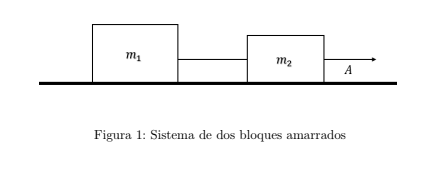
\includegraphics[width=10cm, height=6cm]{diagrama 1.png}
   \subsection*{ Diagrama de cuerpo libre}
     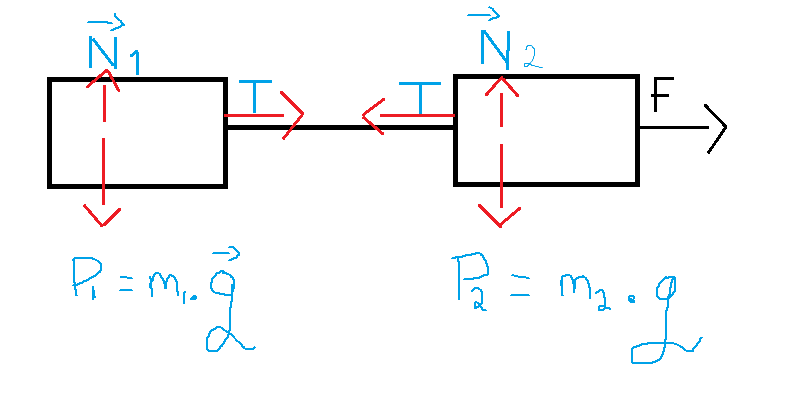
\includegraphics[width=10cm, height=6cm]{diagrama de cuerpo libre.png}\\
Usando segunda ley de Newton $F_{total}$ = $masa\cdot aceleración$\\
Entonces tenemos\\
\begin{align*}
    T= m_1 \cdot a\\
    F-T = m_2 \cdot a
\end{align*}\\
sumamos ambas ecuaciones y obtenemos \\
\begin{align*}
    F-T+T \Rightarrow{F} = m_1 \cedot a + m_2 \cdot a\\
    F= a (m_1+m_2)\\
    a = \frac{F}{m_1+m_2}
\end{align*}
Y como fuerza resultante solo tenemos una\\
\begin{equation*}
   T = M_1 \cdot a
\end{equation*}
\section{Punto extra}
  El paquete hyperref permite crear links entre distintas partes del documento o incluso links a páginas web externas. Es muy útil para crear links entre elementos del texto y el punto del documento donde se encuentra el elemento en cuestión. Con este paquete puede crearse una tabla de contenidos de modo que cada título pueda ser clicado para trasladarse a la página correspondiente.\\
  Para cargarlo, se utiliza la sintaxis habitual:
   usepackage[opciones]{hyperref}
  Para especificar opciones, alternativamente se puede utilizar el comando:
    hypersetup{opcion1=valor1,opcion2=valor2,etc...}
    Uno de los comandos básicos para crear enlaces de hipertexto es:
\href{Tipo:Dirección}{Objeto}
Que asigna un hiperenlace a Objeto, redirigiéndolo a Dirección. Podemos elegir entre
los siguientes tipos:
http Tipo por defecto, que no necesita ser indicado. Tampoco es necesario incluir los
dos puntos ó doble barra que suelen aparecer en las direcciones de internet. Por
ejemplo:
href{www.uva.es}{Universidad de Valladolid}
ftp Para conectar con servidores ftp:
href{ftp://ftp.rediris.es/pub/}{Servidor Rediris}
mailto Para enviar correos electrónicos:
href{mailto:lmolina@fta.uva.es}{Enviar correo al profesor}
file Abre un archivo con el programa asociado:
href{file:c:/camino/archivo}{Nombre del archivo}
run Permite ejecutar aplicaciones:
href{run:c:/windows/notepad.exe}{Abrir el bloc de notas}
Aparte de los hiperenlaces creados automáticamente por hyperref a partir de los
enlaces básicos de LATEX, se pueden incluir hiperenlaces con la pareja de comandos:
hypertarget{etiqueta}{texto de llegada}
hyperlink{etiqueta}{texto del enlace}
Para enlazar con otra página del documento se puede usar:
hyperlink{page.N}{Número de página}
2
que enlazaría con la página N.
 \begin{thebibliography}{1}
 \bibitem[1]Paquetes importantes de LaTeX | Manualdelatex.com. (s. f.). Recuperado 6 de noviembre de 2022, de https://manualdelatex.com/tutoriales/paquetes
 \bibitem[2]Apuntes de LATEX Capítulo 10: Documentos navegables y presentaciones. (s. f.). mat.uda.cl. Recuperado 6 de noviembre de 2022, de https://mat.uda.cl/hsalinas/cursos/2008/latex/apuntes10.pdf
 \end{thebibliography}
\end{document}
